% !TeX program = latexmk
% !TeX spellcheck = pl_PL
% !TeX root = example.tex

\chapter{Implementacja projektu}

Projekt aplikacji wspomagającej zdalne szacowanie historyjek metodą planning pokera został wykonany w technologii webowej o nazwie ReactJS oraz Firebase po stronie backendu. ReactJS to biblioteka javascript stworzona przez firmę Facebook oraz Instagram dzięki której budowanie dużych oraz kompleksowych interfejsów użytkownika jest łatwiejsze. Jest ona przeznaczona do wykorzystania z innym frameworkiem, który wprowadza backend. Podczas gdy Angular, Ember oraz Backpone są popularnymi wyborami do tego, Firebase wprowadza najłatwiejszą i najszybszą integrację z trwałym backendem czasu rzeczywistego do aplikacji napisanej w ReactJS – zajmuje to tylko kilka linijek w Javascript. 

\section{Czym jest ReactJS}

Twórcy ReactJS opisują go jako Widok w architekturze MVC, nie ma na celu zastąpienie Angular’a oraz Ember’a; zamiast tego rozszerza ich funkcjonalność przez wprowadzenie bardzo wydajnej drogi utrzymania widoku zsynchronizowanego z javascript. Ten specjalny sos który renderuje HTML używa wyjątkowo szybkiego algorytmu wirtualnego drzewa DOM, wprowadzający o wiele lepszą wydajność niż konkurujące platformy. Ma jednokierunkowy reaktywny przepływ danych, który jest znacznie bardziej zrozumiały niż tradycyjne przepływy danych. Komponenty – podstawowe bloki aplikacji React-owych – są zorganizowane w drzewie hierarchicznym, w którym komponenty rodzice wysyłają dane do swoich dzieci przez zmienne właściwości. Każdy komponent ma także zmienną stanu, która determinuje obecne dane dla tego widoku. Za każdym razem, gdy stan jest zmieniany, komponent wywołuje metodę render() a React znajduje najbardziej efektywną metodę aktualizacji drzewa DOM.

Odkąd głównym zadaniem React’a jest interfejs użytkownika, aplikacje na nim zrobione potrzebują czegoś jeszcze, co będzie zachowywało się jak backend. To jest miejsce gdzie Firebase wkracza. Dodaje Model i Kontroler w MVC do aplikacji napisanych w ReactJS, czyniąc z nich w pełni funkcjonujące aplikacje. Używając React’owego jednokierunkowego systemu wiązania danych łatwo jest zintegrować go z Firebase.\cite{www_react}

\section{Firebase}

Firebase jest platformą dla aplikacji webowych oraz mobilnych która wprowadza dla deweloperów mnóstwo narzędzi oraz usług by pomóc im tworzyć wysokiej jakości aplikacje oraz zwiększyć ich bazę użytkowników.

\subsection{Historia Firebase}

W 2011 roku, zanim Firebase było Firebase’em był startup nazwany Envelope. Jako Envelope  wprowadził dla deweloperów API, które umożliwiało wprowadzenie czatu do ich strony internetowej.

Interesującym było to, że ludzie używali aplikacji by przekazywać dane, które były czymś więcej niż wiadomościami chatowymi. Deweloperzy używali Envelope by synchronizować dane aplikacji jak stan gry w czasie rzeczywistym pomiędzy ich użytkownikami.

To poprowadziło założycieli Envelope, Jamesa Tamplina oraz Andrew Lee do pomysłu by rozdzielić chat oraz architekturę czasu rzeczywistego. W kwietniu 2012 Firebase został stworzony jako oddzielna firma które wprowadziła Backend jako usługę z funkcjonalnościami czasu rzeczywistego. 

Po tym jak firma została przejęta przez Google w 2014 roku szybko ewoluowała do wielofunkcyjnej platformy mobilnej oraz webowej jaką znamy dzisiaj. rys.\ref{rys:firebase}

% Rysunek
\begin{figure}
\centering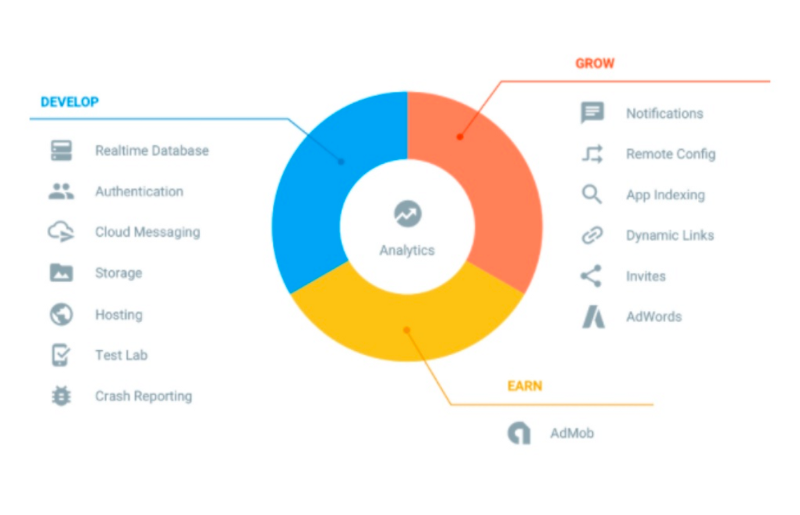
\includegraphics[width=.6\textwidth]{img/firebase}
\caption{Usługi Firebase.[hackernoon.com]}  \label{rys:firebase}% Źródło rysunku i etykieta przez którą odwołujemy się do rysunku.
\end{figure}

\section{Wykorzystane usługi Firebase}

\subsection{Firebase Authentication}

Przede wszystkim w swojej aplikacji skorzystałem z usługi Fierbase Authentication, która wprowadza serwerowe usługi, łatwe narzędzia dla deweloperów oraz gotowe biblioteki interfejsu by wprowadzić usługę logowania i rejestrowania do naszej aplikacji.

Normalnie zajęłoby miesiące by ustawić system autoryzacji na własną rękę. A nawet wtedy twórcy musieliby mieć dedykowany zespół by utrzymywać ten system. Ale jeżeli wykorzystają Firebase’a, mogą ustawić cały system w mniej niż 10 linijek kodu, które zajmą się wszystkim włącznie z kompleksowymi operacjami jak scalanie kont.

W swoim projekcie skorzystałem z usług logowania anonimowego oraz przez Github’a co było kluczowe w moim projekcie.

\subsection{Firestore}

Firestore jest nie relacyjną bazą dokumentów, która pozwala łatwo przechowywać, synchronizować oraz przeszukiwać dane dla aplikacji mobilnych oraz webowych – w globalnej skali.

Firestore przechowuje dane w postaci obiektów zwanych dokumentami. Te dokumenty posiadają pary klucz-wartosć oraz mogą zawierać jakiekolwiek rodzaje danych od łańcuchów po dane binarne a nawet obiekty, które przypominają drzewa JSON. Dokumenty są pogrupowane w kolekcje. rys.\ref{rys:firestoreData}

\begin{figure}
	\centering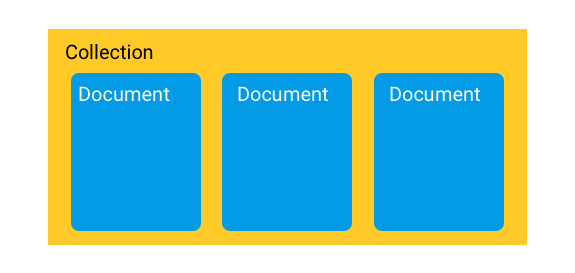
\includegraphics[width=.6\textwidth]{img/firestoreData}
	\caption{Postać danych w firestore [hackernoon.com]}\label{rys:firestoreData}% Źródło rysunku i etykieta przez którą odwołujemy się do rysunku.
\end{figure}

Fierstore może zawierać wiele kolekcji zawierających dokumenty, które wskazują na subkolekcje. Te subkolekcje mogą znowu zawierać dokumenty oraz sub kolekcje i tak dalej.
Można zatem powiedzieć że w tym modelu danych wszystko jest ułożone chierarchicznie.\cite{www_hakermoon}
rys.\ref{rys:firestoreTree}

\begin{figure}
	\centering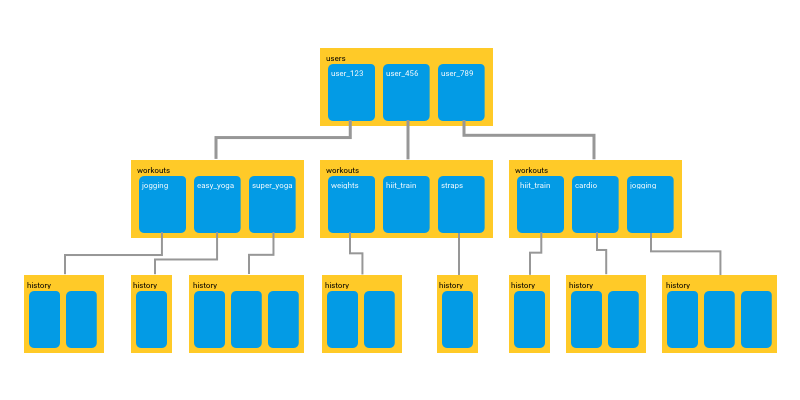
\includegraphics[width=.6\textwidth]{img/firestoreTree}
	\caption{Ułożenie danych w firestore [hackernoon.com]}\label{rys:firestoreTree}% Źródło rysunku i etykieta przez którą odwołujemy się do rysunku.
\end{figure}

\section{Redux czyli implementacja architektury Flux.}

Jedną z najważniejszych cech komponentów ReactJS jest wbudowany w nie stan. Jest to bardzo przydatny koncept. Komponent posiada stan, który może ulec zmianie w wyniku interakcji użytkownika z aplikacją. Zmiana stanu pociąga za sobą operację re-renderowania drzewa Virtual DOM. W wyniku tego, pewne części interfejsu widocznego na ekranie ulegają zmianie. Oczywiście wiadomym jest też, że jeden komponent może zależeć od innego komponentu. Możemy przecież przekazywać stan komponentu rodzica do jego komponentów dzieci itd.
To wszystko działa świetnie. Niestety w miarę jak aplikacja rośnie, rozrasta się poziom skomplikowania poszczególnych komponentów. Z tego względu programiści Facebooka odpowiedzialni za rozwój ReactJS wymyślili architekturę aplikacji, która rozwiązuje ten problem. Architektura ta nazwa się Flux.\cite{www_nafrontendzie}

\subsection{Architektura FLUX}

Flux jest architekturą aplikacji którą Facebook używa do budowania aplikacji po stronie klienta. Jest to uzupełnienie komponentów React’a przez wykorzystanie jednokierunkowego przepływowi danych. To jest raczej pewien wzorzec niż framework i można z niego korzystać  bez wielu nowych linijek kodu. rys. \ref{rys:flux}

\begin{figure}
	\centering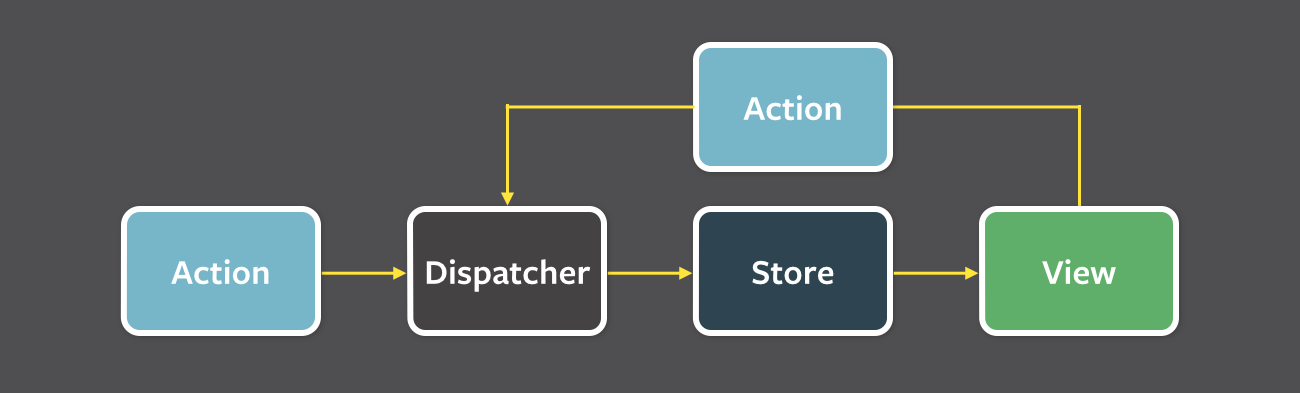
\includegraphics[width=.6\textwidth]{img/flux}
	\caption{architektura flux [wwww.nafrontendzie.pl]}\label{rys:flux}% Źródło rysunku i etykieta przez którą odwołujemy się do rysunku.
\end{figure}

Przepływ rozpoczyna się od lewej strony. Najpierw tworzone jest akcja – jest to zwykły obiekt zawierający właściwość type. Oprócz tego może on posiadać więcej właściwości służących do przekazywania dodatkowych danych. Akcja taka tworzona jest przez funkcję zwaną action creator czyli kreator akcji. W przypadku redux'a jednak akcja jest zwykłą funkcją. Listing \ref{listing:licznik}

% lub {java} albo {bash} albo {text}
\begin{listing}
\begin{minted}{c}
const mapStateToProps = (state) => {
return { counter: state.counter };
};
const mapDispatchToProps = (dispatch) => {
return {
onIncrement: () => dispatch({ type: 'INCREMENT' }),
onDecrement: () => dispatch({ type: 'DECREMENT' })
}
};

Counter = connect(mapStateToProps, mapDispatchToProps)(Counter);
\end{minted}
\caption{Przykładowe akcje licznika i ich stan} \label{listing:licznik}
\end{listing}

W tym przykładzie przedstawiony jest przykład prostego licznika z dwoma akcjami, które albo zwiększają albo zmniejszają licznik o jeden. Stan oraz funkcję rozsyłające dostępne są w obiekcie this.props. Spójrzmy na kod odpowiedzialny za ich mapowanie.
\begin{center}
	\textbf{Funkcja mapStateToProps}
\end{center}
Funkcja \textit{mapStateToProps} pobiera \textit{state} jako parametr i zwraca nowy obiekt. Częstą praktyką jest po prostu przekazanie całego stanu do `propsów`, jednak jest to też właściwe miejsce by odfiltrować dane. 
\begin{center}
	\textbf{Funkcja mapDispatchToProps}
\end{center}
Kolejna funkcja to \textbf{mapDispatchToProps}. Zwraca ona obiekt zawierający metody. Za pomocą wywołania funkcji \textbf{dispatch} rozgłasza ona obiekty akcji do \textbf{store}. W powyższym przykładzie mamy pewne uproszczenie: do metody dispatch przekazywane obiekty akcji przekazywane są bezpośrednio. Zwykle w projekcie definiuje się to jako specjalne kreatory akcji. Dzięki kreatorom możemy opóźnić wywołanie akcji, lub zmienić dane w naszym redux'ie tylko wtedy, gdy są spełnione określone warunki. Listing \ref{listing:firebase_action}

% lub {java} albo {bash} albo {text}
\begin{listing}
	\begin{minted}{c}
	export const startAddUserToGame = (owner, repo, game, user = {}) => {
	return dispatch => {
	var userUpdate = {}
	const tempUser = {
	email: user.email,
	isAnonymous: user.isAnonymous,
	id: user.uid,
	name: user.displayName,
	online: true
	};
	userUpdate[`users.` + user.uid.toString()] = tempUser
	const gameRef = db
	.collection(`users`)
	.doc(owner.toString())
	.collection(`repos`)
	.doc(repo.toString())
	.collection(`games`)
	.doc(game.toString())
	
	gameRef.update(userUpdate).then(() => {
	dispatch(addUserToGame(owner, repo, game, tempUser))
	});
	}
	}
	\end{minted}
	\caption{Przykładowy kreator akcji z projektu} \label{listing:firebase_action}
\end{listing}

W tym przykładzie gracz jest dodawany do gry, tylko wtedy, kiedy jest dodany do gry w bazie danych firestore. Jak widać w przykładzie kreator zwraca funkcję, która wykorzystuje dyspatch by wysłać akcję do store. Aby zadziałać funkcja musi znać dokładną lokalizację gry w bazie oraz dane użytkownika. Aby dostać się do gry, musimy znać właściciela oraz nazwę repozytorium w której znajduje się gra, a później identyfikator gry. Później dodajemy gracza do naszej gry dzięki funkcji update dostając się odpowiednio do kolekcji użytkownicy, dokumentu użytkownika, kolekcji repozytoria, dokumentu naszego repozytorium. Później z repozytoriów wchodzimy do kolekcji gier, a dzięki znajomości identyfikatora gry dostajemy się do obiektu gry i wstawiamy do obiektu gry obiekt gracza. Jeżeli akcja w bazie danych zakończy się sukcesem rozsyłamy akcję dodawania gracza do store.
\begin{center}
	\textbf{Funkcja connect}
\end{center}
Ale wróćmy do tematu mapowania. W przedstawionym wcześniej przykładzie najbardziej istotna jest ostatnia jego linia. Jak widzisz, wywołuję w niej funkcję connect. Przyjmuje ona funkcje mapStateToProps oraz mapDispatchToProps jako parametry i wyniki ich wywołania łączy w odpowiedni obiekt. Następnie zwraca ona funkcję, która jako parametr przyjmuje komponent. Funkcja ta wstrzykuje przygotowany wcześniej obiekt do this.props tego komponentu.

Zwróć też uwagę, że ostateczny wynik opisanych działań jest przypisywany ponownie do obiektu komponentu. To dlatego, że funkcja zwracana przez funkcję connect opakowuje przekazany komponent i zwraca nową jego wersję.

Wróćmy teraz do FLUX. Tak tworzona akcja jest dostarczana do store za pomocą wywołania funkcji zwaną dispatcher. Funkcja ta w zasadzie zarządza całym przepływem danych. Każdy store w aplikacji rejestruje w dispatcherze swoje funkcje wywołania zwrotnego w celu obsługi przychodzących akcji. W momencie gdy akcja jest rozsyłana (ang. dispatch), wywoływane są po kolei wszystkie te callbacki. Jeden z nich powinien umieć rozpoznać akcję po jej typie i być przygotowany na jej odpowiednią obsługę.

\begin{center}
	\textbf{Funkcja reducer}
\end{center}

W przypadku redux'a role store'a pełni funkcja \textbf{reducer}. Dzięki temu, że jest to funkcja , można ją jednocześnie użyć jako funkcję wywołania zwrotnego, którą store uruchomi w momencie gdy zostanie rozgłoszona jakaś akcja. Funkcja ta przyjmuje dwa parametry: \textbf{state} oraz \textbf{action}

Generalnie działa to tak: ktoś wywołuje akcję, obiekt \textbf{store} wywołuje funkcję \textbf{reducer}, przekazując do niej aktualny stan oraz akcję, funkcja \textbf{reducer} sprawdza typ przekazanej do niej akcji i w zależności jak jest ten typ, zwraca nową wersję obiektu stanu. Przykład: Listing \ref{listing:reducer} 

\begin{listing}
	\begin{minted}{c}
	const reducer = (state, action) => {
	switch (action.type) {
	case 'INCREMENT':
	return { ...state, counter: state.counter + 1 };
	case 'DECREMENT':
	return { ...state, counter: state.counter - 1 };
	default:
	return state;
	}
	};
	\end{minted}
	\caption{Przykładowy reducer licznika} \label{listing:reducer}
\end{listing}

W przykładzie, jeśli typ akcji to `INCREMENT` to zwracany jest nowy obiekt stanu, który ma zwiększoną o jeden wartość atrybutu counter. Jeśli natomiast typ akcji to `DECREMENT` to zwracany jest nowy stan z atrybutem counter zmniejszonym o jeden. Jeśli natomiast typ akcji jest zupełnie inny, obiekt stanu jest po prostu przekazywany dalej.

Generalnie wszystkie obiekty store zawierają łącznie cały stan aplikacji. Store zawiera implementację funkcji wywoływania zwrotnego, która jest rejestrowana w „dispatcherze”, i która obsługuje akcję związane z danym store.
W redux'ie cały stan jest przechowywany w jednym obiekcie.

Kolejny element na diagramie to widok. Można powiedzieć, że jest on reprezentowany po prostu przez komponent ReactJS. Używa on stanu aplikacji zapisanego w obiekcie store, tak jakby był on wewnętrznym stanem komponentu. Zmiana stanu w store powoduje re-renderownie komponentu. Dodatkowo komponent widoku może rozsyłać kolejne akcje, na przykład kiedy użytkownik kliknie na jakiś guzik na ekranie. To powoduje zmianę stanu zapisanego w store.
W redux'ie komponent ma dostęp do akcji i stanu dzięki wspomnianej przeze mnie wcześniej funckji connect.

Wszystko to po prostu zestaw zasad. To programista może zdecydować jak to dokładnie będzie zaimplementowane. Na szczęście nie jest on zdany sam na siebie poniewać istnieje kilka gotowych implementacji architektury Flux w postaci bibliotek.\cite{www_nafrontendzie}
Jedną z nich jest oczywiście redux.

\subsection{Czym redux różni się od Flux}

Redux jest inspirowany pewnymi ważnymi cechami architektury Flux. Tak jak Flux Redux przepisuje twój model danych do oddzielnej warstwy twojej aplikacji (“stores” in Flux, “reducers” in Redux). Tak jak we Flux wszystkie operacji na danych są opisywane w postaci akcji. W przeciwieństwie do Flux Redux nie ma konceptu rozsyłacza, ponieważ opiera się na czystych funkcjach zamiast emiterów akcji, a czyste funkcje są łatwe do tworzenia i nie potrzebują żadnej encji by zarządzać nimi. Jest to więc pewne odstępstwo od Flux’a.\cite{www_nafrontendzie} 

Inną ważną różnicą od Flux’a jest to że Redux zakłada że dane są niemutowalne. Możesz używać używać statycznych obiektów oraz tablic dla swojego stanu, ale mutowanie ich wewnątrz reducerów jest silnie nie rekomendowana. Zawsze powinieneś zawsze zwracać nowy obiekt. Ogólnie Redux może być opisany przez trzy fundamentalne zasady:
rys.\ref{rys:reduxFlux}
\begin{itemize}
	\item Pojedyncze źródło prawdy - stan całej aplikacji przetrzymywany jest w drzewie obiektów wewnątrz pojedynczego obiektu store.
	\item Stan jest tylko do odczytu - jedynym sposobem na zmianę stanu jest wywołanie akcji, która zwraca obiekt opisujący co powinno się stać.
	\item Zmiany wykonywane są w ramach czystych funkcji - aby określić jak drzewo stanu transformowane jest przez akcje musisz tworzyć “czyste reducery”.
\end{itemize}

\begin{figure}
	\centering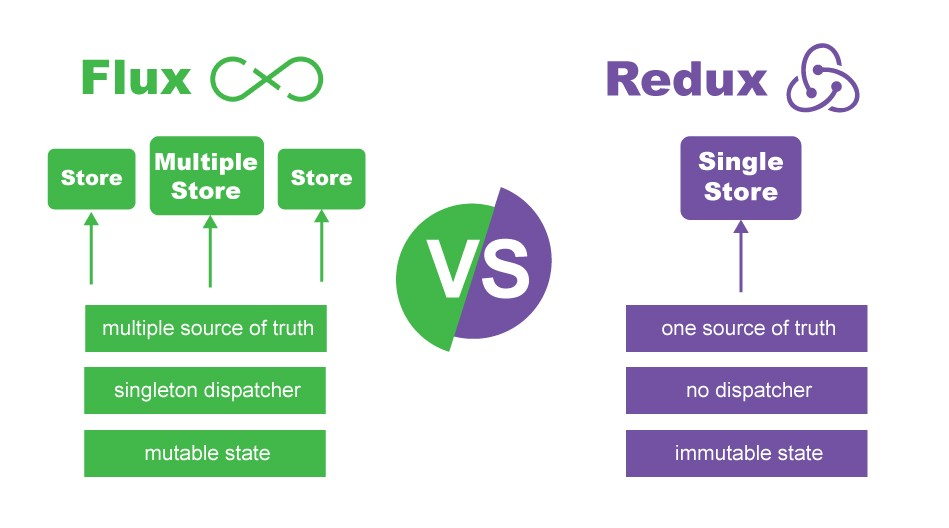
\includegraphics[width=.6\textwidth]{img/reduxFlux}
	\caption{Różnice między Redux a Flux [www.medium.com]}\label{rys:reduxFlux}% Źródło rysunku i etykieta przez którą odwołujemy się do rysunku.
\end{figure}

\subsection{redux-thunk}

Biblioteka redux-thunk została stworzona przaz Dana Abramova, który jednocześnie jest twórcą Reduxa. Pozwala ona tworzyć kreatory akcji, które zamiast obiektu zwracają funkcję. Dzięki temu możliwe jest opóźnienie rozgłoszenia akcji lub zgłoszenie jej tylko jeśli zostaną spełnione określone warunki.\cite{www_thunk} Jak dodać thunk do reduxa: Listing \ref{listing:thunk-redux}

\begin{listing}
	\begin{minted}{c}
	import { createStore, applyMiddleware } from 'redux';
	import thunk from 'redux-thunk';
	import rootReducer from './reducers/index';
	
	const store = createStore(
	rootReducer,
	applyMiddleware(thunk)
	);
	\end{minted}
	\caption{Połączenie reduxa i thunka} \label{listing:thunk-redux}
\end{listing}

\newpage

\begin{center}
	\textbf{Obsługa wywołań asynchronicznych - kreatory akcji}
\end{center}

W przykładzie listing \ref{listing:firebase_action} przedstawiłem akcję, która najpierw dodaje użytkownika do bazy a później rozgłasza akcję dodawania użytkownika, jeżeli modyfikacja danych w bazie zakończyła się pomyślnie. W funkcji \textbf{startAddUserToGame} pobierane są najpierw dane o grze, czyli: \textbf{owner}, który jest po prostu identyfikatorem użytkownika githuba, który jest właścicielem repozytorium, którego nazwa jest w zmiennej \textbf{repo}. Następnie jest pobierany identyfikatory gry (\textbf{game}). Na końcu dostajemy dane użytkownika, którego chcemy dodać do gry. Funkcja ta zwraca funkcję przyjmującą parametr \textbf{dispatch}, który służy do rozgłaszania danych. Później jest tworzony użytkownik, który ma zostać dodany do gry (\textbf{temUser}). Na końcu jest tworzony obiekt, będący odnośnikiem do użytkowników w bazie, który pomaga zaktualizować obiekt gry. Później jest tworzona referencja do obiektu gry w bazie danych (\textbf{gameRef}). Później korzystając z referencji aktualizuje się obiekt gry w bazie danych, a w razie sukcesu (funkcja \textbf{then}) akcja jest rozsyłana dalej.

\subsection{Połączenie Firebase i redux’a
}

Jak nie trudno się domyśleć wszystkie operacje pomiędzy Firebase a Redux są realizowane w postaci akcji. Do synchronizacji Frontend’u z backend’em służy thunk, który przesyła dane do store’a tylko wtedy, kiedy nie ma żadnych problemów po stronie firebase’a. Jeżeli baza danych nie będzie mogła pobrać danych z bazy bo wystąpił błąd, thunk nie wykona operacji. Sposób połączenia tych dwóch elementów przedstawiono na rys. \ref{rys:fireRedux} 

\begin{figure}
	\centering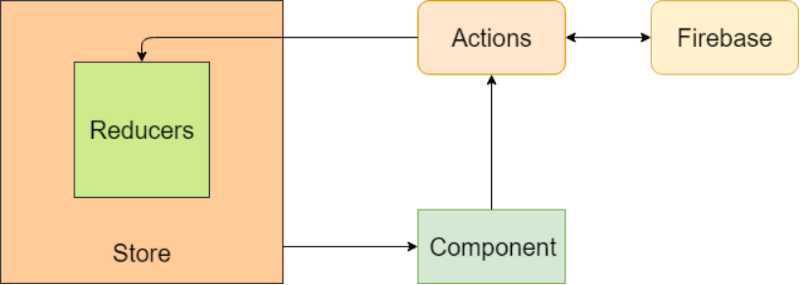
\includegraphics[width=.6\textwidth]{img/fireRedux}
	\caption{Sposób połączenia firebase i reduxa. [medium.com]}\label{rys:fireRedux}% Źródło rysunku i etykieta przez którą odwołujemy się do rysunku.
\end{figure}
